\documentclass[11pt, a4paper]{article}

%%%%%%%%%%%%%%%%%
% Configuration %
%%%%%%%%%%%%%%%%%
\usepackage{allrunes}
\usepackage{amsmath}
% If magyar is wanted
% \usepackage[magyar]{babel}
\usepackage[T1]{fontenc}
\usepackage[utf8]{inputenc}
\usepackage{fixltx2e}
\usepackage{multirow}
\usepackage{url}
\usepackage{amsfonts}
\usepackage{amsthm}
\usepackage{mathtools}
\usepackage{amssymb}
\usepackage{xcolor}

% feynman diagrams
\usepackage{tikz-feynman}

% using circled symbols
\usepackage{tikz}
\newcommand*\circled[1]{\tikz[baseline=(char.base)]{
            \node[shape=circle,draw,inner sep=2pt] (char) {#1}}}


% Here you can configure the layout
\usepackage{geometry}
\geometry{top=1cm, bottom=1cm, left=1.25cm,right=1.25cm, includehead, includefoot}
\setlength{\columnsep}{7mm} % Column separation width

\usepackage{graphicx}

%\usepackage{gensymb}
\usepackage{float}

% For bra-ket notation
\usepackage{braket}

% To have a good appendix
\usepackage[toc,page]{appendix}

\usepackage{abstract}
\renewcommand{\abstractnamefont}{\normalfont\bfseries}
\renewcommand{\abstracttextfont}{\normalfont\small\itshape}
\usepackage{lipsum}

%%%%%%%%%%%%%%%%%%%
% Custom commands %
%%%%%%%%%%%%%%%%%%%
\newcommand{\bb}[1]{\mathbf{#1}}
\newcommand{\dd}{\mathrm{d}}
\newcommand{\Tr}[1]{\mathrm{Tr}\left[#1\right]}
\newcommand{\Sp}[1]{\mathrm{Sp}\left[{#1}\right]}

% \newtheorem*{tetel*}{Tétel}
% \newtheorem*{defn*}{Definíció}
% \newtheorem*{pld*}{Példa}
% \newtheorem*{megj*}{Megjegyzés}
% \newtheorem*{allit*}{Állítás}

% \newtheorem{tetel}{Tétel}
% \newtheorem{defn}{Definíció}
% \newtheorem{pld}{Példa}
% \newtheorem{megj}{Megjegyzés}
% \newtheorem{allit}{Állítás}

% Hyperref should be generally the last package to load
% Any configuration that should be done before the end of the preamble:

\usepackage{hyperref}
\hypersetup{colorlinks=true, urlcolor=blue, linkcolor=blue, citecolor=blue}

\title{Flowering date prediction for bulbous perennials}

\author{Dániel Nagy$^1$,\\Imre M. Jánosi$^2$}
\vspace{2.0cm}
\date{%
    $^1$Institute for Physics, Eötvös Loránd University, H-1117, Pázmány Péter sétány 1/A. Budapest, Hungary\\%
    $^2$Department of Physics of Complex Systems, Eötvös Loránd University, H-1117, Pázmány Péter sétány 1/A. Budapest, Hungary\\[2ex]%
    \today
}

\begin{document}
\maketitle
\vspace{2.5cm}
\begin{figure}[H]
    \centering
    
\includegraphics[scale=0.3]{images/elte.eps}
\end{figure}
\vspace{0.5cm}

\newpage
\begin{abstract}
    The goal of this project is to efficiently predict the first flowering date of bulbous perennials and to identify,
    which meteorological parameters affect the flowering dates. The LSCD model is briefly presented, and the hyperparameters
    of the simpler LSC model are fitted using Gaussian process optimization. A neural network approach for the
    prediction of flowering dates is presented.
\end{abstract}

\section*{Introduction}
\par Many observations prove that plants have a complex sense of climate, and that many of them developed the ability
to prevent premature flowering.
In order to uncover the relationship between meteorological data and flowering time, a long-term data acquisition was needed.
The data available to my project is a \texttt{csv} file that is containing the first flowering dates of 329 bulbous perennial plants 
in the period 1968-2001. Further meteorological data is downloaded from the internet. The most significant meteorological parameter 
is the temperature of the soil at a depth of around 10cm. The temperature data is shown on \ref{fig:tempdata}.
\begin{figure}[H]
    \centering
    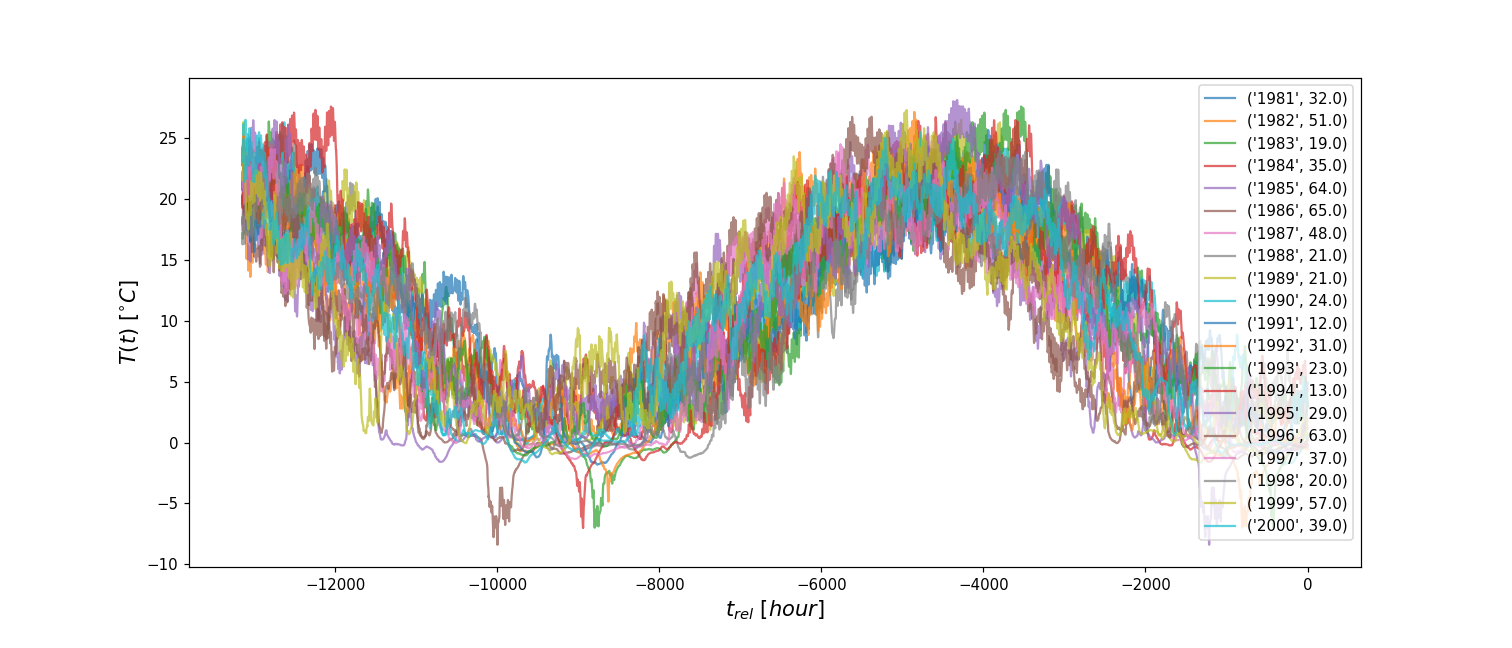
\includegraphics[width=0.75\textwidth]{images/temp_plot.png}
    \caption{The soil temperature at 10cm depth across 22 years, plotted yearly at a 1-hour resolution.
    The x axis shows the hours before flowering date starting from 0.}
    \label{fig:tempdata}
\end{figure}

\section*{The LSCD model}
The LSCD model is built upon the observation that the flowering time of plants is highly correlated with the concentration 
of the Vernalization insensitive3 (VIN3) protein. The  VIN3 mRNA levels are slowly rising with increasing weeks of cold exposure
but rapidly decrease in the warm. Equations \ref{eq:diffnu} and \ref{eq:diffV} describe the 
dynamics of spliced and unspliced VIN3 mRNA concentration.
\begin{equation}
    \frac{\mathrm d\nu}{\mathrm d t} = p_{\nu}(L, S, C, D) - s_{\nu}\nu
    \label{eq:diffnu}
\end{equation}
\begin{equation}
    \frac{\mathrm dV}{\mathrm dt} = s_{\nu}\nu - d_VV
    \label{eq:diffV}
\end{equation}
In the equations above, 
$p_{\nu}(L, S, C, D)=L\cdot S\cdot C\cdot D$ is the productive transcription,
$s_{\nu}$ is the splicing rate, and $d_V$ is the degradation rate of the spliced VIN3.

According to the model, the VIN3 concentration is determined by 4 different intermediators
called the Long-term, the Short-term, the Current and the Diurnal intermediator proteins.
The concentration of these intermediators are described by equations \ref{eq:dLdt}-\ref{eq:Dt}.
\begin{equation}
    \frac{\mathrm dL}{\mathrm dt} =
    \begin{cases}
    1-d_LL & T < T_L \\
    -d_LL & T \geq T_L
    \end{cases}
    \label{eq:dLdt}
\end{equation}

\begin{equation}
    C(T) =
    \begin{cases}
    p_{c1} & T \leq T_{c1} \\
    p_{c1}-p_{c2}\frac{T-T_{c1}}{T_{c2}-T_{c1}} & T_{c1} < T < T_{c2} \\
    p_{c2} & T \geq T_{c2}
    \end{cases}
    \label{eq:CT}
\end{equation}

\begin{equation}
    S(T_m) = 
    \begin{cases}
    1, & T < T_S \\
    S_1, & T \geq T_S
    \end{cases}
    \label{eq:STm}
\end{equation}

\begin{equation}
    D(t) =  \left[p_D + \sin\left(2\pi\left(t - \frac{t_m-1}{24}\right)\right)\right]^2
    \label{eq:Dt}
\end{equation}
$T_m$ is the maximum temperature since the last resetting, which was chosen to occur each day at 4pm.
$t_m$ is the time at dawn.
\begin{figure}[H]
    \centering
    \begin{minipage}{0.4\textwidth}
        \centering
        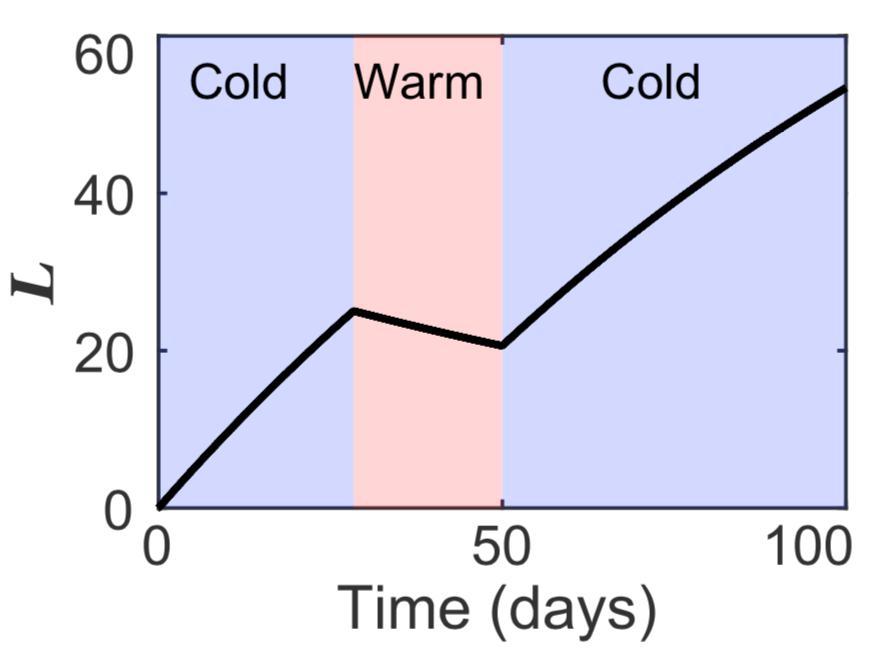
\includegraphics[width=1.0\textwidth]{./images/param_L.png}
        \caption{Illustration of change of $L$ as a function of time and temperature.}
        \label{fig:param_L}
    \end{minipage}
    \hfill
    \begin{minipage}{0.4\textwidth}
        \centering
        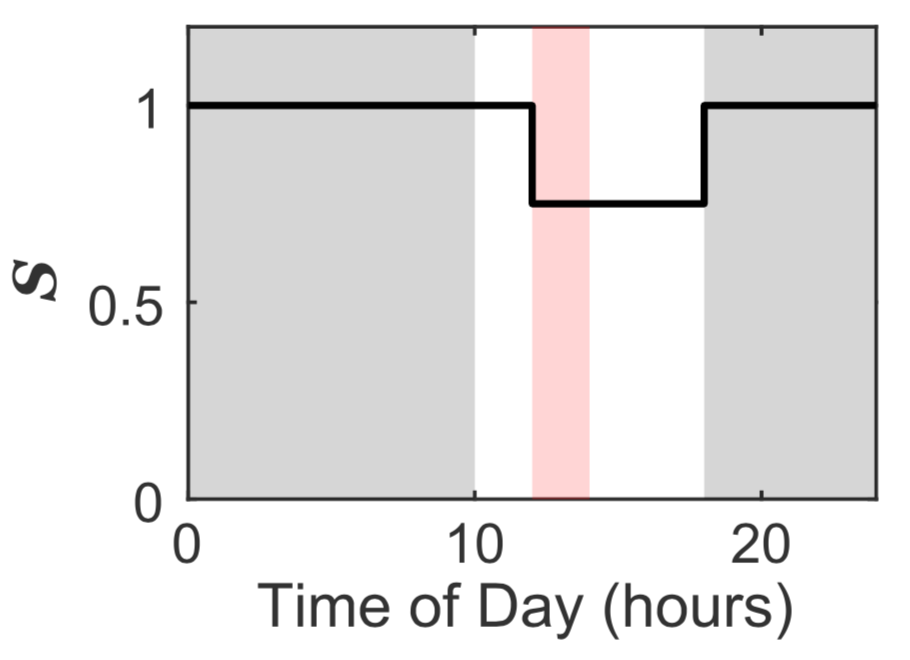
\includegraphics[width=1.0\textwidth]{./images/param_S.png}
        \caption{Illustration of change of $S$ as a function of time and temperature.}
        \label{fig:param_S}
    \end{minipage}
\end{figure}
\begin{figure}[H]
    \centering
    \begin{minipage}{0.4\textwidth}
        \centering
        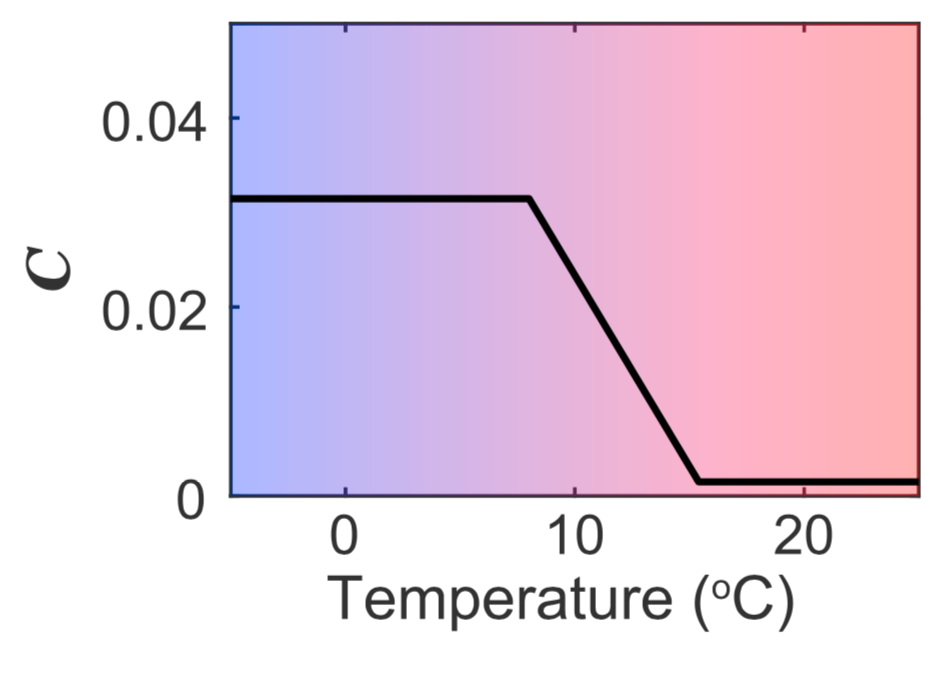
\includegraphics[width=1.0\textwidth]{./images/param_C.png}
        \caption{Illustration of change of $C$ as a function of time and temperature.}
        \label{fig:param_C}
    \end{minipage}
    \hfill
    \begin{minipage}{0.4\textwidth}
        \centering
        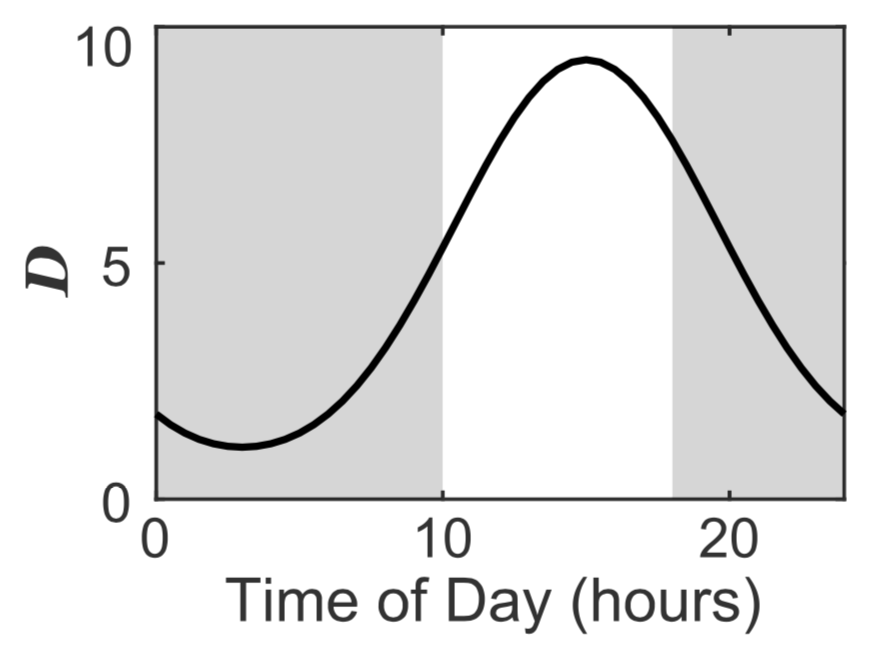
\includegraphics[width=1.0\textwidth]{./images/param_D.png}
        \caption{Illustration of change of $D$ as a function of time and temperature.}
        \label{fig:param_D}
    \end{minipage}
\end{figure}
Figures \ref{fig:param_L}-\ref{fig:param_D} show how the intermediator levels are changing with the temperature and time.
\subsection*{Results with the LSCD model}
I investigated the LSCD model for a single type of bulbous perennial for a 20-year dataset. 
\begin{figure}[H]
    \centering
    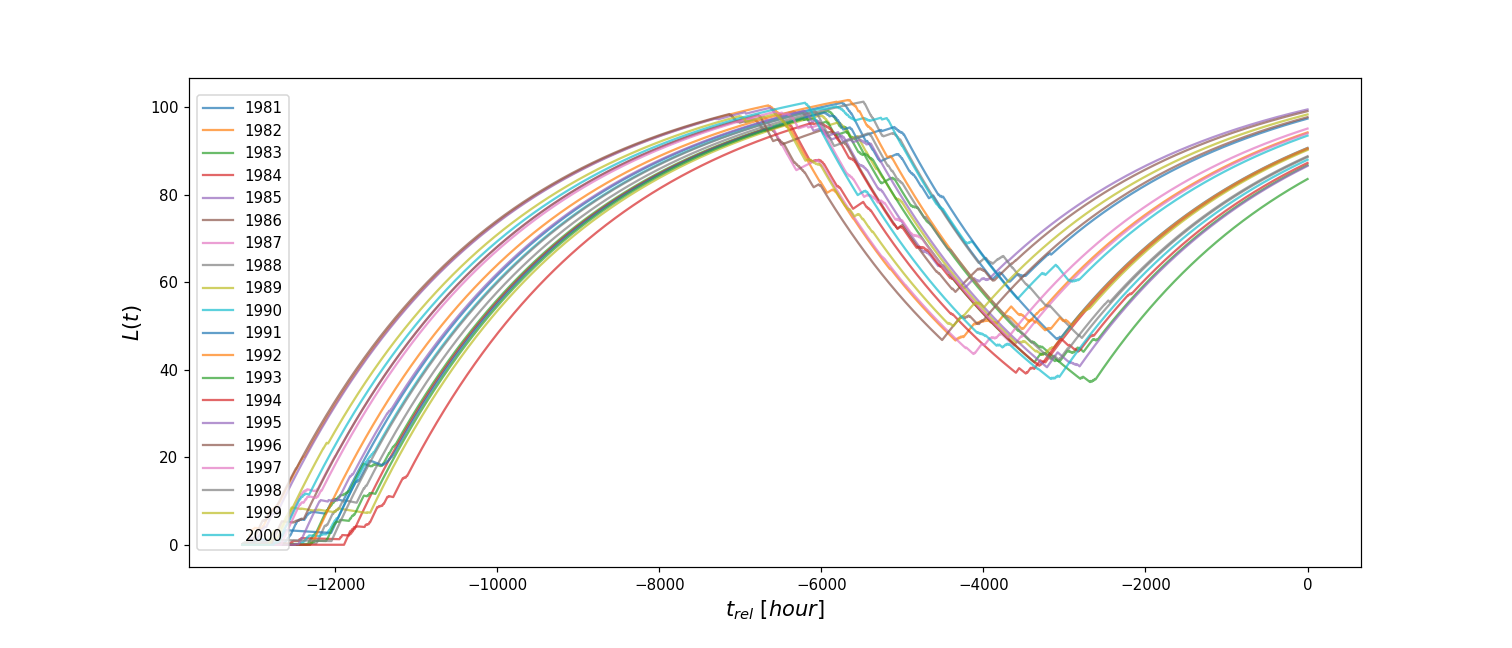
\includegraphics[width=0.75\textwidth]{images/L_plot.png}
    \caption{$L$ intermediator for a one-year period temperature data across 20 years.}
\end{figure}
\begin{figure}[H]
    \centering
    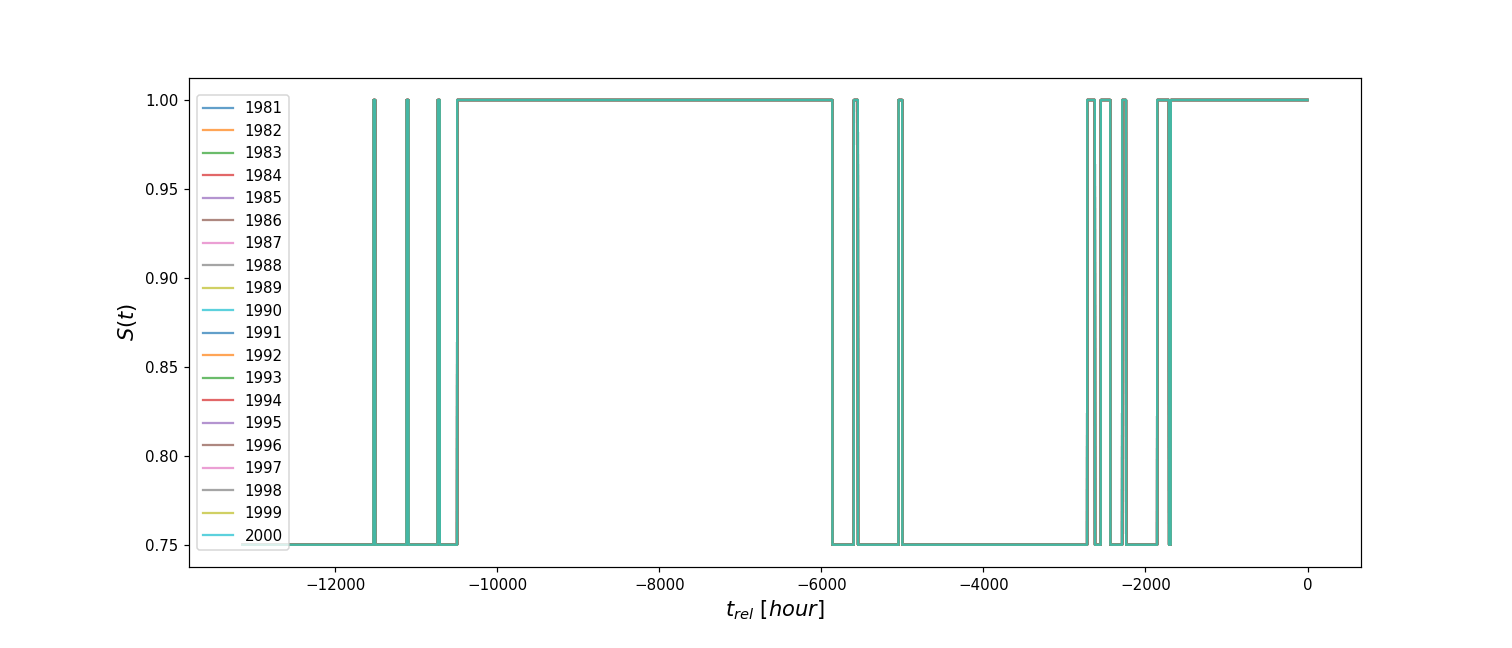
\includegraphics[width=0.75\textwidth]{images/S_plot.png}
    \caption{$S$ intermediator for a one-year period temperature data across 20 years.}
\end{figure}
\begin{figure}[H]
    \centering
    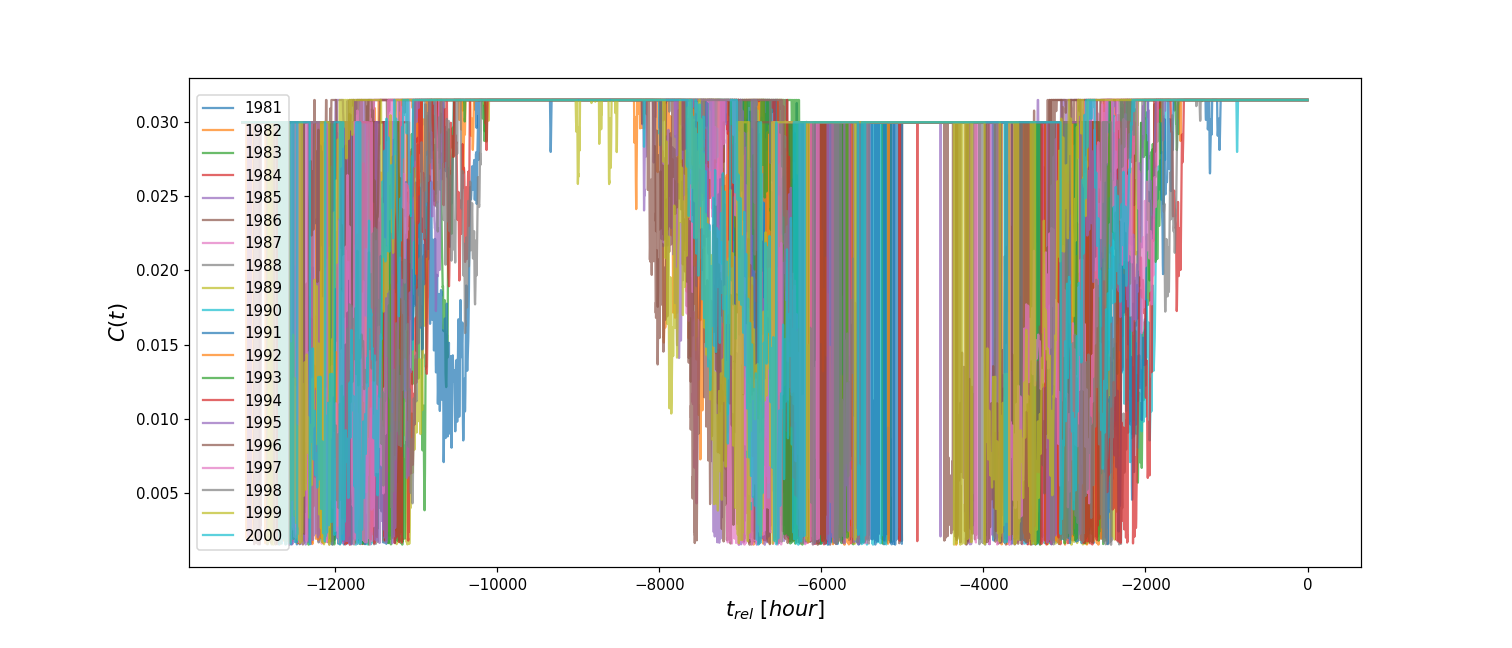
\includegraphics[width=0.75\textwidth]{images/C_plot.png}
    \caption{$C$ intermediator for a one-year period temperature data across 20 years.}
\end{figure}
\begin{figure}[H]
    \centering
    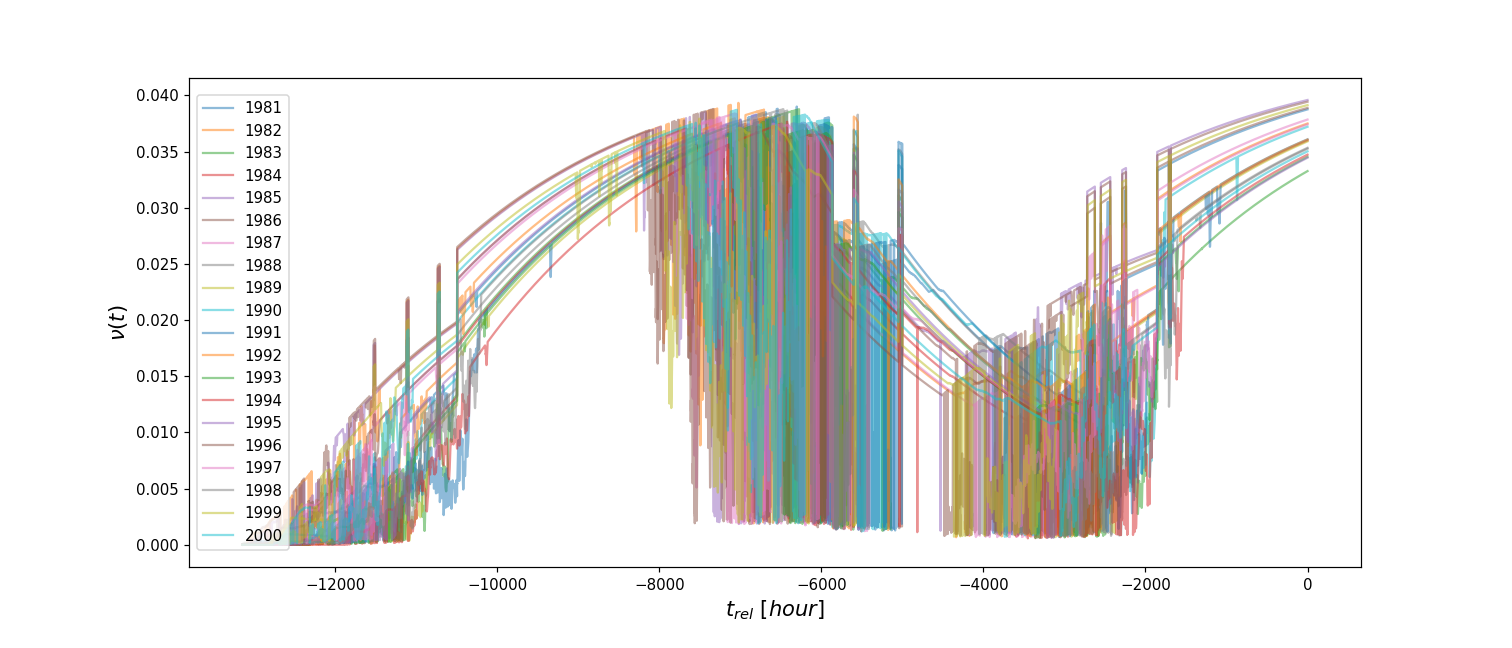
\includegraphics[width=0.75\textwidth]{images/nu_plot.png}
    \caption{Spliced VIN3 concentration for a one-year period temperature data across 20 years.}
\end{figure}
\subsection*{Gaussian process optimization}
The hyperparamteres of the simpler LSC model were searched with Gaussian process optimization using the \texttt{scikit-optimize}
python package. The results of the fit are shown on figures \ref{fig:LSC_skopt_evals} and \ref{fig:LSC_skopt_objective}.
\begin{table}[H]
    \centering
    \begin{tabular}{|c|c|c|c|}
    \hline
    param & dimension  & initial value & fitted value \\ \hline
    $d_V$     & day$^{-1}$& 18 & 19.7069 \\ \hline
    $s_{\nu}$ & day$^{-1}$& 79.2 & 70.655 \\ \hline
    $S_1$     & 1 & 0.75 & 2.1732 \\ \hline
    $T_L$     & $^{\circ}$C & 17 & 31.945 \\ \hline
    $d_L$     & day$^{-1}$& 0.009 & 0.074249 \\ \hline
    $T_{c1}$  & $^{\circ}$C & 8 & 10.1501 \\ \hline
    $T_{c2}$  & $^{\circ}$C & 15.4 & 14.4630 \\ \hline
    $p_{c1}$  & 1 & 0.0315 & 0.01038 \\ \hline
    $p_{c2}$  & 1 & 0.03   & 0.0309 \\ \hline
    $p_D$     & 1 & 2.05 & - \\ \hline
    $T_S$     & $^{\circ}$C & 15 &17.164 \\ \hline
    \end{tabular}
    \caption{Values of the parameters in the literature and values after applying GP optimizer on the LSC model.}
\end{table}

\begin{figure}[H]
    \centering
    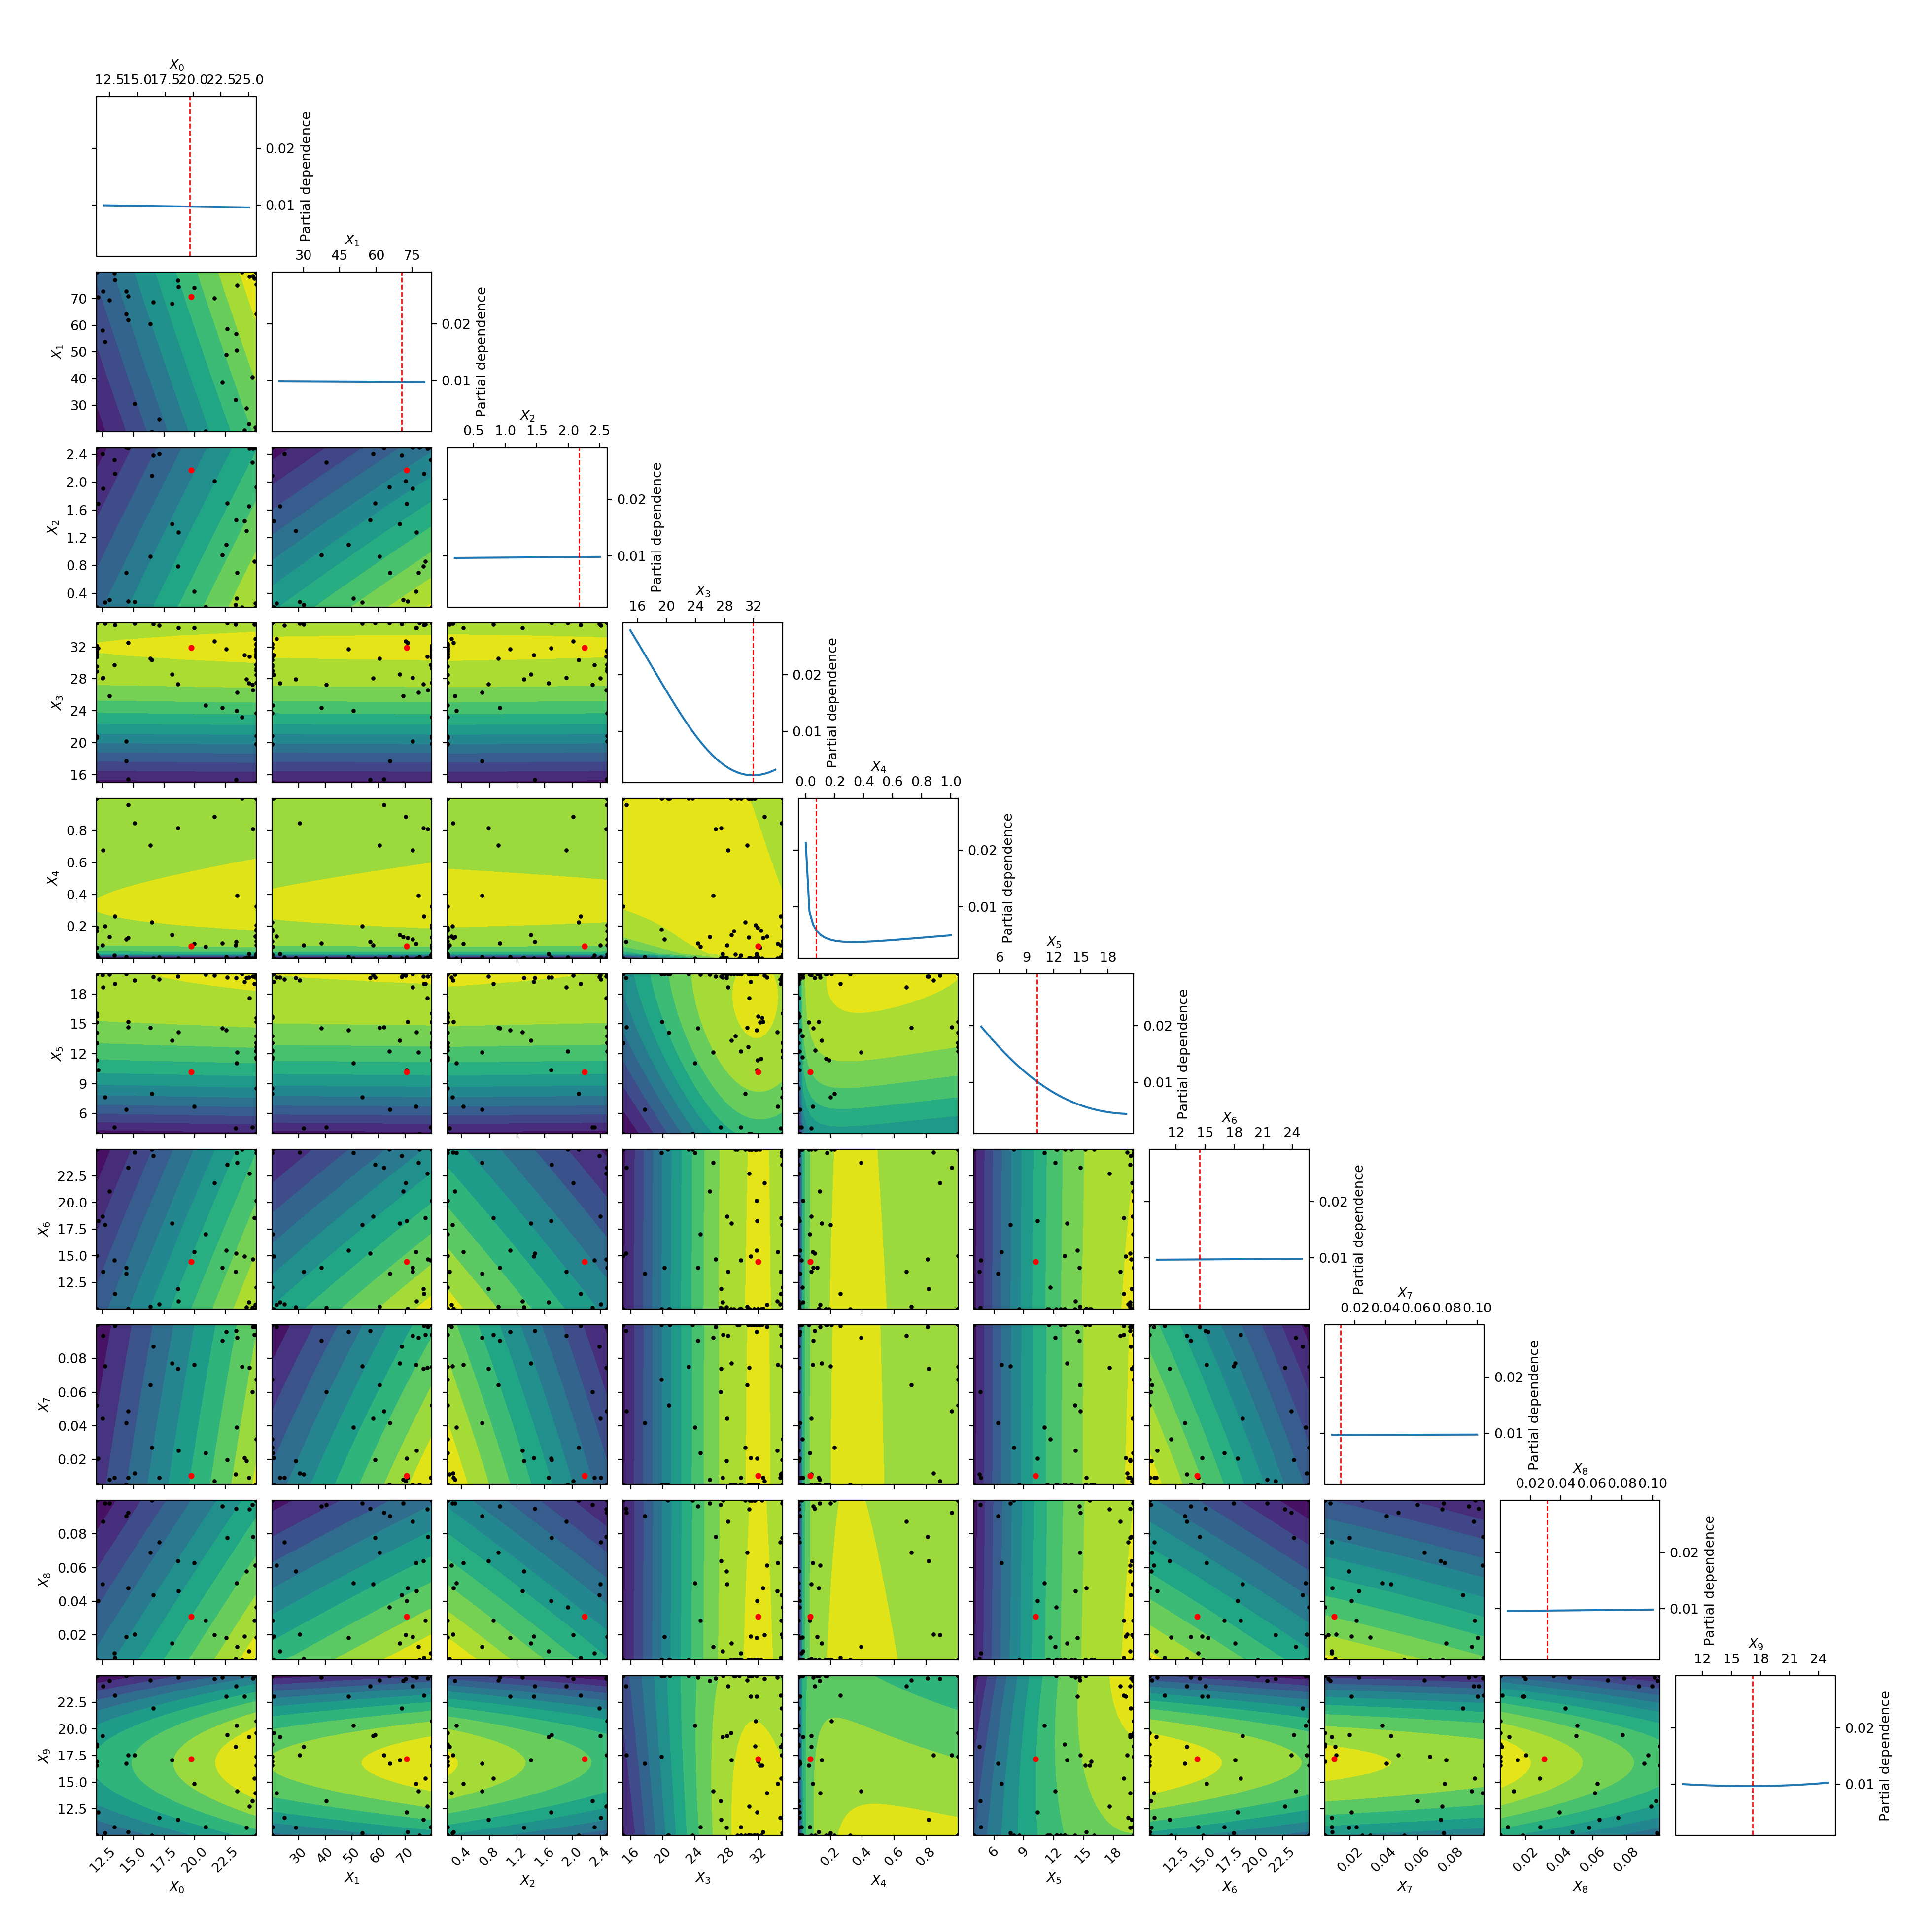
\includegraphics[width=0.99\textwidth]{images/LSC_skopt_objective.png}
    \caption{Results of objectives of the LSC model while fitting parameters with the GP optimizer.}
    \label{fig:LSC_skopt_objective}
\end{figure}

\begin{figure}[H]
    \centering
    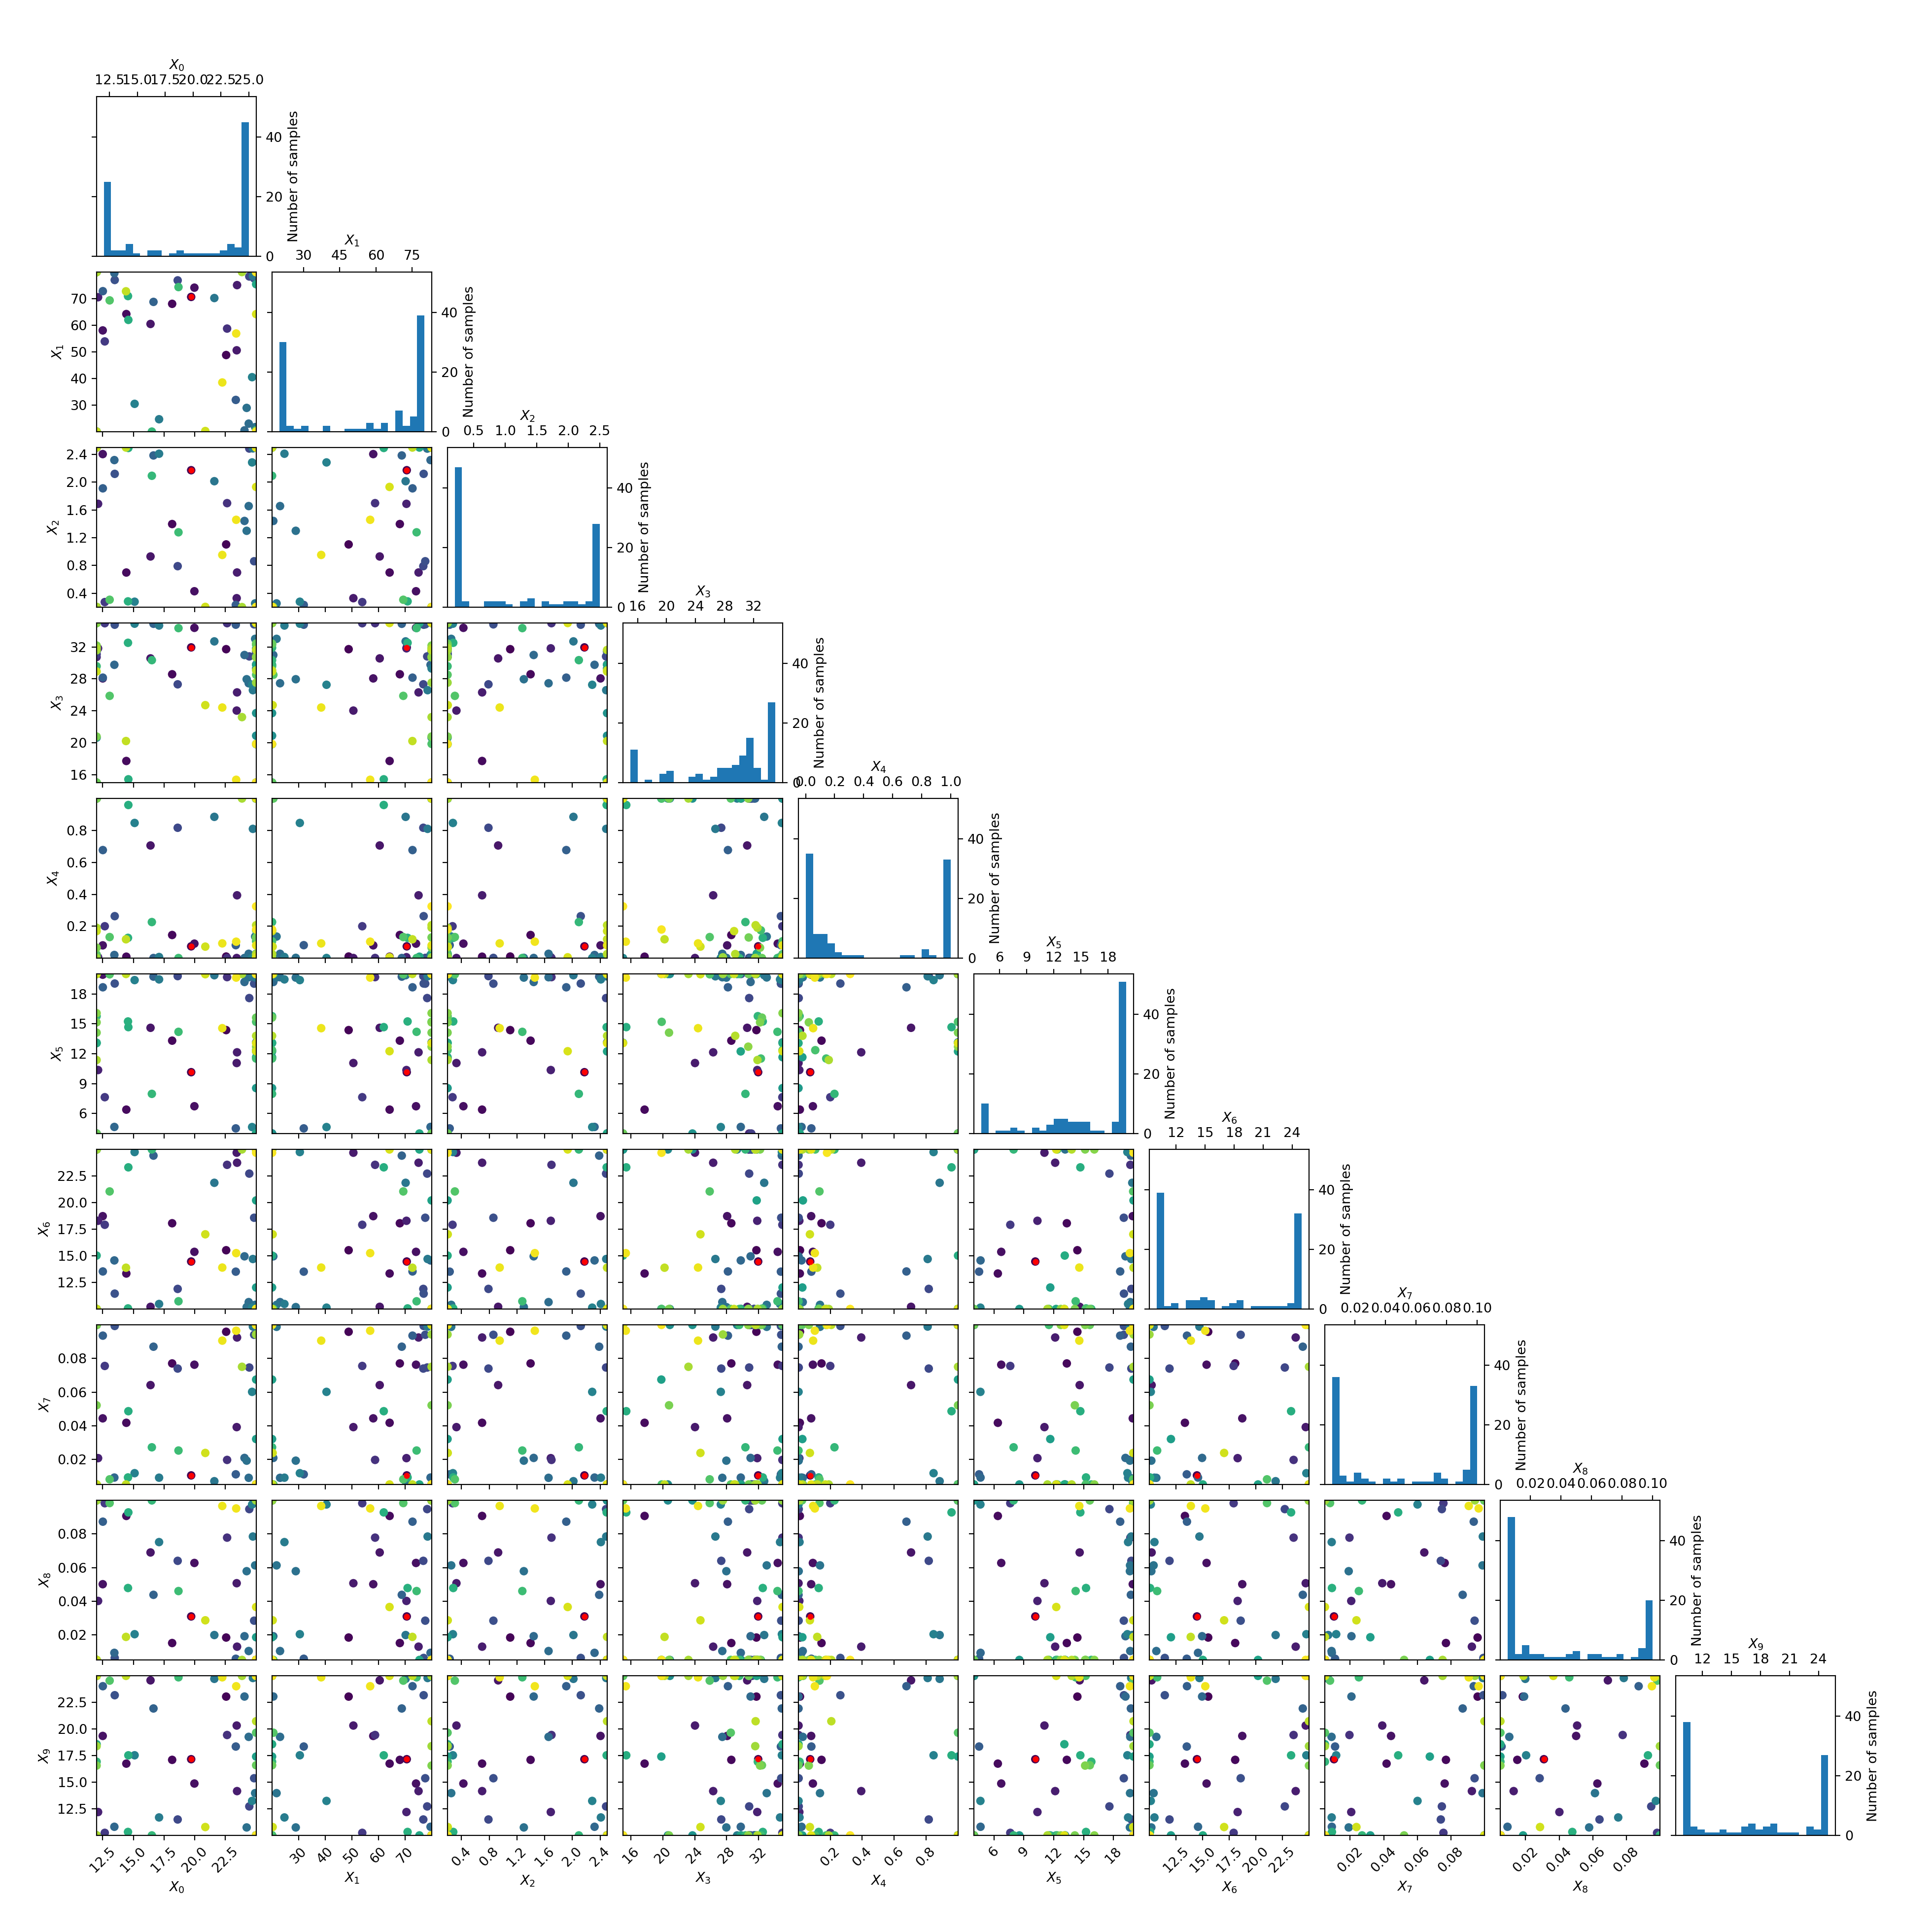
\includegraphics[width=0.99\textwidth]{images/LSC_skopt_evals.png}
    \caption{Results of evaluations of the LSC model with the GP optimizer.}
    \label{fig:LSC_skopt_evals}
\end{figure}


\newpage
\section*{Neural network approach}
A neural network was implemented aiming to predict the time until the next flowering date bassed on a sequence of temperature
measurement data. The network was feeded with a dataset created by systematically resampling the existing temperature series and 
labeling these sequances. The architecture is based on LSTM cells and was a single layer recursive neural network. 
The schema of this architecture is seen on figure \ref{fig:LSTM_arch}.
\begin{figure}[H]
    \centering
    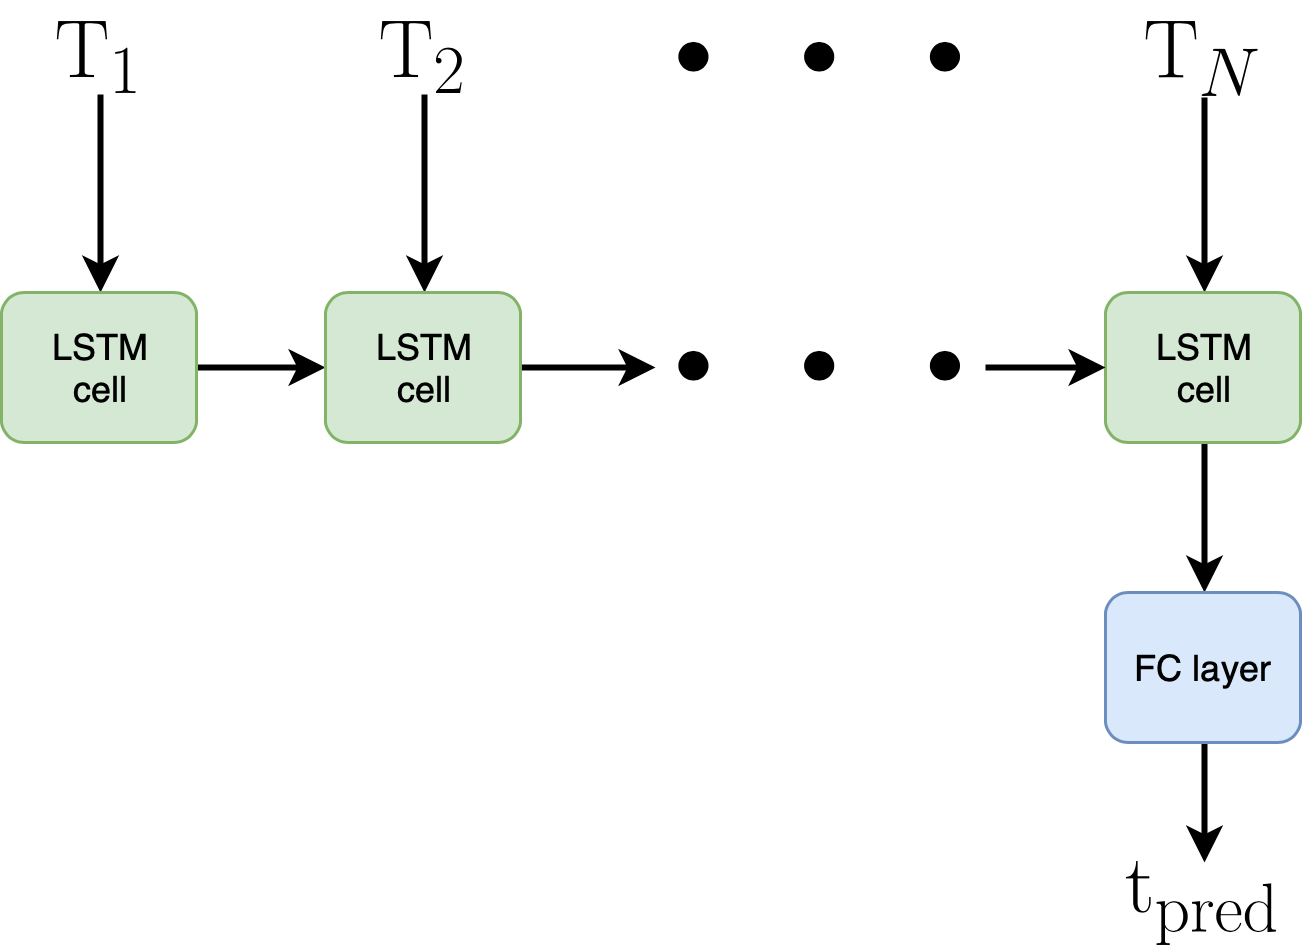
\includegraphics[width=0.45\textwidth]{images/LSTM_arch.png}
    \caption{LSTM architecture for predicting flowering time from temperature measurement series.}
    \label{fig:LSTM_arch}
\end{figure}
The LSTM cells have cell state of 16 float values and also a hidden state of 16 floats. At the end there is a fully connected 
layer equipped with ReLU activation to predict a single float value.
\subsection*{Results of the neural network approach}
The network was trained on a part of the available data with batch size 8. The model was trained for 300 epochs with
Adam optimizer and the learning rate was set to 0.03. Figure \ref{fig:loss-6} show the loss during training.
\begin{figure}[H]
    \centering
    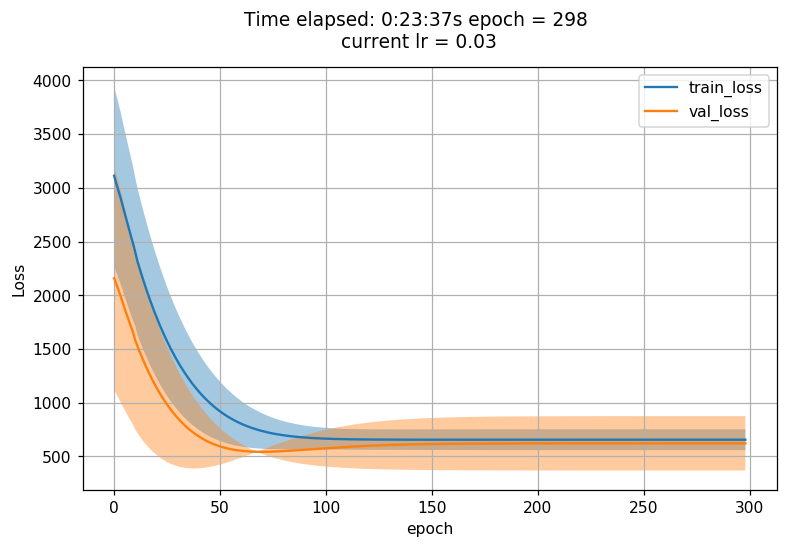
\includegraphics[width=0.6\textwidth]{images/loss-6.png}
    \caption{Loss functions on training and validation datasets across 300 epochs.}
    \label{fig:loss-6}
\end{figure}
Altough the model was converging, the mean squared error is still large, meaning that it is plenty of room for improvement.
The fact that this simple model was converging even for a small subset of the data, without overfitting, gives hope that
significant improvement could be achieved in the future.

\end{document}